\PassOptionsToPackage{unicode=true}{hyperref} % options for packages loaded elsewhere
\PassOptionsToPackage{hyphens}{url}
%
\documentclass[]{book}
\usepackage{lmodern}
\usepackage{amssymb,amsmath}
\usepackage{ifxetex,ifluatex}
\usepackage{fixltx2e} % provides \textsubscript
\ifnum 0\ifxetex 1\fi\ifluatex 1\fi=0 % if pdftex
  \usepackage[T1]{fontenc}
  \usepackage[utf8]{inputenc}
  \usepackage{textcomp} % provides euro and other symbols
\else % if luatex or xelatex
  \usepackage{unicode-math}
  \defaultfontfeatures{Ligatures=TeX,Scale=MatchLowercase}
\fi
% use upquote if available, for straight quotes in verbatim environments
\IfFileExists{upquote.sty}{\usepackage{upquote}}{}
% use microtype if available
\IfFileExists{microtype.sty}{%
\usepackage[]{microtype}
\UseMicrotypeSet[protrusion]{basicmath} % disable protrusion for tt fonts
}{}
\IfFileExists{parskip.sty}{%
\usepackage{parskip}
}{% else
\setlength{\parindent}{0pt}
\setlength{\parskip}{6pt plus 2pt minus 1pt}
}
\usepackage{hyperref}
\hypersetup{
            pdftitle={CM 2110 Calculus and Statistical Distributions},
            pdfauthor={Dr.~Priyanga D. Talagala},
            pdfborder={0 0 0},
            breaklinks=true}
\urlstyle{same}  % don't use monospace font for urls
\usepackage{longtable,booktabs}
% Fix footnotes in tables (requires footnote package)
\IfFileExists{footnote.sty}{\usepackage{footnote}\makesavenoteenv{longtable}}{}
\usepackage{graphicx,grffile}
\makeatletter
\def\maxwidth{\ifdim\Gin@nat@width>\linewidth\linewidth\else\Gin@nat@width\fi}
\def\maxheight{\ifdim\Gin@nat@height>\textheight\textheight\else\Gin@nat@height\fi}
\makeatother
% Scale images if necessary, so that they will not overflow the page
% margins by default, and it is still possible to overwrite the defaults
% using explicit options in \includegraphics[width, height, ...]{}
\setkeys{Gin}{width=\maxwidth,height=\maxheight,keepaspectratio}
\setlength{\emergencystretch}{3em}  % prevent overfull lines
\providecommand{\tightlist}{%
  \setlength{\itemsep}{0pt}\setlength{\parskip}{0pt}}
\setcounter{secnumdepth}{5}
% Redefines (sub)paragraphs to behave more like sections
\ifx\paragraph\undefined\else
\let\oldparagraph\paragraph
\renewcommand{\paragraph}[1]{\oldparagraph{#1}\mbox{}}
\fi
\ifx\subparagraph\undefined\else
\let\oldsubparagraph\subparagraph
\renewcommand{\subparagraph}[1]{\oldsubparagraph{#1}\mbox{}}
\fi

% set default figure placement to htbp
\makeatletter
\def\fps@figure{htbp}
\makeatother

\usepackage{booktabs}
\usepackage{amsthm}
\makeatletter
\def\thm@space@setup{%
  \thm@preskip=8pt plus 2pt minus 4pt
  \thm@postskip=\thm@preskip
}
\makeatother
\usepackage{fancyhdr}
\pagestyle{fancy}
\fancyfoot[CO,CE]{Prepared by Dr. Priyanga D. Talagala}
\fancyfoot[LE,RO]{\thepage}
\usepackage{wrapfig}
\usepackage{floatrow}
\floatplacement{figure}{H}
\floatplacement{table}{H}
\makeatletter\renewcommand*{\fps@figure}{H}\makeatother
\usepackage{mathtools}
\usepackage[]{natbib}
\bibliographystyle{apalike}

\title{CM 2110 Calculus and Statistical Distributions}
\author{Dr.~Priyanga D. Talagala}
\date{2020-05-29}

\begin{document}
\maketitle

{
\setcounter{tocdepth}{1}
\tableofcontents
}
\hypertarget{course-syllabus}{%
\chapter*{Course Syllabus}\label{course-syllabus}}
\addcontentsline{toc}{chapter}{Course Syllabus}

\hypertarget{pre-requisites}{%
\section*{Pre-requisites}\label{pre-requisites}}
\addcontentsline{toc}{section}{Pre-requisites}

CM 1110

\textbf{Remark:}

\emph{This course module contains two main sections: (1) mathematics and (2) statistics. This syllabus is designed for the statistics section. Lectures for mathematics section and statistics section are conducted by two lecturers as two separate sub modules (1.5 hour lectures/Week). End Semester Examination is conducted as a single examination.}

\hypertarget{learning-outcomes}{%
\section*{Learning Outcomes}\label{learning-outcomes}}
\addcontentsline{toc}{section}{Learning Outcomes}

On successful completion of this module, students will be able to plan more carefully the design of experiment in advance which provide evidence for or against theories of cause and effect and make inferences about population characteristics based on sample information and thereby solve data analysis problems in different application domains. (R(\url{https://cran.r-project.org/}) and RStudio are also freely available to install on your own computer). Get the Open Source Edition of RStudio Desktop. RStudio allows you to run R in a more user-friendly environment.

\hypertarget{outline-syllabus}{%
\section*{Outline Syllabus}\label{outline-syllabus}}
\addcontentsline{toc}{section}{Outline Syllabus}

\begin{itemize}
\tightlist
\item
  Functions of Several Variables
\item
  Linear Algebra
\item
  Coordinate Systems \& Vectors
\item
  Differential Equations
\item
  \textbf{Statistical Distributions}
\item
  \textbf{Estimation}
\item
  \textbf{Hypothesis Testing}
\item
  \textbf{Design of Experiments}
\end{itemize}

\hypertarget{method-of-assessment}{%
\section*{Method of Assessment}\label{method-of-assessment}}
\addcontentsline{toc}{section}{Method of Assessment}

\begin{itemize}
\tightlist
\item
  Mid-semester examination
\item
  End-semester examination
\end{itemize}

\hypertarget{recommended-texts}{%
\section*{Recommended Texts}\label{recommended-texts}}
\addcontentsline{toc}{section}{Recommended Texts}

\begin{itemize}
\tightlist
\item
  Casella, G., \& Berger, R. L. (2002). Statistical inference (Vol. 2, pp.~337-472). Pacific Grove, CA: Duxbury.
\item
  Mood, A.M., Graybill, F.A. and Boes, D.C. (2007): Introduction to the Theory of Statistics, 3rd Edn.
  (Reprint). Tata McGraw-Hill Pub. Co.~Ltd.~
\item
  Montgomery, D. C. (2017). Design and analysis of experiments. John wiley \& sons.
\end{itemize}

\hypertarget{lecturer}{%
\section*{Lecturer}\label{lecturer}}
\addcontentsline{toc}{section}{Lecturer}

Dr.~Priyanga D. Talagala

\hypertarget{schedule}{%
\section*{Schedule}\label{schedule}}
\addcontentsline{toc}{section}{Schedule}

Lectures:

\begin{itemize}
\tightlist
\item
  Friday {[}9.15 am - 10.45 am{]}
\end{itemize}

Tutorial:

\begin{itemize}
\tightlist
\item
  Friday {[}11.00 am - 12.30 pm{]}
\end{itemize}

Consultation time:

\begin{itemize}
\tightlist
\item
  Friday {[}8.15 am to 9.00 am{]}
\end{itemize}

\hypertarget{statistical-distributions}{%
\chapter{Statistical Distributions}\label{statistical-distributions}}

\pagenumbering{arabic}

\hypertarget{recap-cm-1110-probability}{%
\section*{Recap: CM 1110-Probability}\label{recap-cm-1110-probability}}
\addcontentsline{toc}{section}{Recap: CM 1110-Probability}

\hypertarget{axioms-of-probability}{%
\subsection*{Axioms of probability}\label{axioms-of-probability}}
\addcontentsline{toc}{subsection}{Axioms of probability}

\begin{center}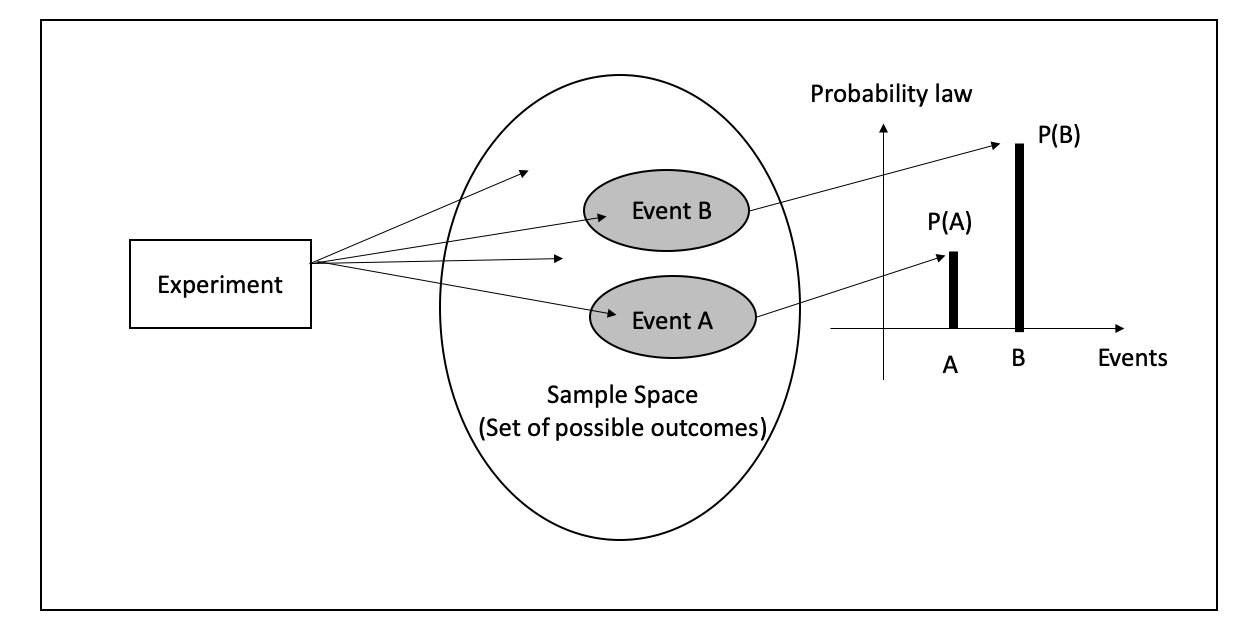
\includegraphics[width=1\linewidth]{figure/Axioms} \end{center}

\begin{itemize}
\item
  \textbf{Probability} of an event quantifies the \textbf{uncertainty}, randomness, or the possibility of occurrence the event.
\item
  The probability of event E is usually denoted by \(P(E)\).
\item
  Mathematically, the function \(P(.)\) is a set function defined from sample space \((\Omega)\) to \([0, 1]\) interval, satisfying the following properties.
\item
  These are called the \textbf{`axioms of probability'}.
\item
  \textbf{Axiom 1:} For any event \(A\), \(P(A) \geq 0\)
\item
  \textbf{Axiom 2:} \(P(\Omega) = 1\)
\item
  \textbf{Axiom 3:}

  \begin{itemize}
  \item
    \begin{enumerate}
    \def\labelenumi{(\alph{enumi})}
    \tightlist
    \item
      If \(A_1, A_2, \dots, A_k\) is a finite collection of mutually exclusive events, then \[P(A_1\cup A_2\cup \dots \cup A_k)= \sum_{i=1}^kP(A_i)\]
    \item
      If \(A_1, A_2, \dots\) is an infinite collection of mutually exclusive events, then
      \[P(A_1\cup A_2\cup \dots)= \sum_{i=1}^\infty P(A_i)\]
    \end{enumerate}
  \end{itemize}
\end{itemize}

\textbf{NOTE}

\begin{itemize}
\tightlist
\item
  Axioms 1 and 2 imply that for any event \(E\), \(0 \leq P (E) \leq 1\).
\item
  \(P (E) = 1 \iff\) the event E is certain to occur.
\item
  \(P (E) = 1 \iff\) the event E cannot occur.
\end{itemize}

\hypertarget{methods-for-determining-probability}{%
\subsection*{Methods for determining Probability}\label{methods-for-determining-probability}}
\addcontentsline{toc}{subsection}{Methods for determining Probability}

\begin{itemize}
\tightlist
\item
  There are several ways for determining the probability of events.
\item
  Usually we use the following methods to obtain the probability of events.

  \begin{itemize}
  \tightlist
  \item
    Classical method
  \item
    Relative frequency method (Empirical approach)
  \item
    Subjective method
  \item
    \textbf{Using probability models}
  \end{itemize}
\end{itemize}

\newpage

\hypertarget{random-variable}{%
\section{Random Variable}\label{random-variable}}

\begin{itemize}
\tightlist
\item
  Some sample spaces contain quantitative (numerical) outcomes, others contain qualitative outcomes.
\item
  Often it is convenient to work with sample spaces containing numerical outcomes.
\item
  A function that maps the original sample space into the real numbers is called a `random variable'.
\item
  This is more useful when the original sample space contains qualitative outcomes.
\end{itemize}

\textbf{Definition 1: Random Variable}

Let \(\Omega\) be a sample space. Let \(X\) be a function from \(\Omega\) to \(\Re\) (\emph{i.e.} \(X:\Omega \rightarrow \Re\)). Then \(X\) is called a random variable.

\begin{center}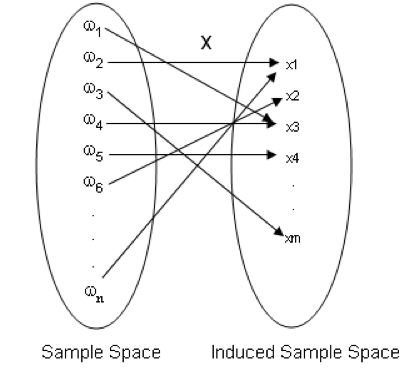
\includegraphics[width=0.5\linewidth]{figure/Ch1_F1} \end{center}

\begin{itemize}
\tightlist
\item
  A random variable assigns a real number to each outcome of a sample space.
\item
  In other words, to each outcome of an experiment or a sample point \(\omega_i\), of the sample spaces, there is a unique real number \(x_i\), known as the value of the random variable \(X\).
\item
  The range of the random variable is called the \emph{induced sample space}.
\item
  \emph{A note on notation:} Random variables will always denoted with uppercase letters and the realized values of the random variable (or its range) will be denoted by the corresponding lowercase letters. Thus, the random variable \(X\) can take the value \(x\).
\item
  Each outcome of a sample space occurs with a certain probability. Therefore, each possible value of a random variable is associated with a probability.
\item
  Any events of a sample space can be written in terms of a suitably defined random variable.
\end{itemize}

\hypertarget{types-of-random-variables}{%
\subsection{Types of Random Variables}\label{types-of-random-variables}}

\begin{itemize}
\tightlist
\item
  A random variable is of two types

  \begin{itemize}
  \tightlist
  \item
    Discrete Random Variable
  \item
    Continuous Random Variable
  \end{itemize}
\end{itemize}

\hypertarget{discrete-random-variable}{%
\subsubsection{Discrete Random Variable}\label{discrete-random-variable}}

\begin{itemize}
\tightlist
\item
  If the induced sample space is discrete, then the random variable is called a \textbf{discrete random variable}.
\end{itemize}

\emph{Example 01}
Consider the experiment of tossing a coin. Express the following events using a suitably defined random variable

\(H=\) \emph{The event of getting a head}

\(T=\) \emph{The event of getting a tail}

\begin{center}
\includegraphics[width=1\linewidth]{figure/Ch1box1-1} \end{center}

\emph{Example 02}

Consider the experiment of rolling of a die. Express the following events using a suitably defined random variable

\(A=\) \emph{The event that the number faced up is less than 5}

\(B=\) \emph{The event that the number faced up is even}

\(C=\) \emph{The event that the number faced up is is 2 or 5}

\begin{center}
\includegraphics[width=1\linewidth]{figure/Ch1box2-1} \end{center}

\newpage

\emph{Example 03}

Consider the experiment of tossing a coin 10 times. Then the sample space \(\Omega\) contains \(2^{10} = 1024\) outcomes. Each outcome is a sequence of 10 H's and T's.

Express the following events in terms of a suitably defined random variable.

\(D=\) \emph{The event that the number of heads is 5}

\(E=\) \emph{The event that the number of tails is less than 4}

\begin{center}
\includegraphics[width=1\linewidth]{figure/Ch1box3-1} \end{center}

\hypertarget{continuous-random-variable}{%
\subsubsection{Continuous Random Variable}\label{continuous-random-variable}}

\begin{itemize}
\tightlist
\item
  If the induced sample space is continuous, then the random variable is called a \textbf{continuous random variable.}
\end{itemize}

\emph{Example 04}

Consider the experiment of measuring the lifetime (in hours) of a randomly selected bulb. Express the following events in terms of a suitably defined random variable.

\(F=\) \emph{The event that the lifetime is less than 300 hours}

\(G=\) \emph{The event that the lifetime is 1000 hours}

\begin{center}
\includegraphics[width=1\linewidth]{figure/Ch1box4-1} \end{center}

\hypertarget{probability-mass-function}{%
\section{Probability Mass Function}\label{probability-mass-function}}

\label{sec:pmf}

\textbf{Definition 2: Discrete density function of a discrete random variable}

If \(X\) is a discrete random variable with distinct values \(x_1, x_2, \dots, x_n, \dots,\) then the function, denoted by \(f_X(.)\) and defined by

\begin{equation}
f_X(x) =
\begin{cases} 
P(X=x) & \text{if } x=x_j, j=1,2,\dots,n,\dots\\
0 & \text{if } x \neq x_j
\end{cases}
\end{equation}

is defined to be the discrete density function of \(X\).

\begin{itemize}
\tightlist
\item
  The values of a discrete random variable are often called \emph{mass points.}
\item
  \(f_X(x)\) denotes the \emph{mass} associated with the \emph{mass point} \(x_j\).
\item
  \textbf{\emph{Probability mass function}} \emph{discrete frequency function} and \emph{probability function} are other terms used in place of \emph{discrete density function}
\item
  Probability function gives the measure of probability for different values of \(X\).
\end{itemize}

\hypertarget{properties-of-a-probability-mass-function}{%
\subsection{Properties of a Probability Mass Function}\label{properties-of-a-probability-mass-function}}

\begin{itemize}
\tightlist
\item
  Let \(X\) be a discrete random variable with probability mass function \(f_X(x)\). Then,
\end{itemize}

\begin{enumerate}
\def\labelenumi{\arabic{enumi}.}
\tightlist
\item
  For any \(x\in \Re\), \(0\leq f_X(x) \leq 1.\)
\item
  Let \(E\) be an event and \(I= \{X(\omega):\omega \in E\}.\) Then \(P(E) = P(X\in I) = \sum_{x \in I}f_X(x).\)
\item
  Let \(R = \{X(\omega):\omega \in \Omega\}.\) Then \(\sum_{x\in \Re} f_X(x) = 1.\)
\end{enumerate}

\hypertarget{representations-of-probability-mass-functions}{%
\subsection{Representations of Probability Mass Functions}\label{representations-of-probability-mass-functions}}

\emph{Example 05}

Consider the experiment of tossing a fair coin. Let

\begin{equation}
X =
\begin{cases} 
0 & \text{if the outcome is a Tail }\\
0 & \text{if the outcome is a Head}
\end{cases}
\end{equation}

Find the probability mass function of \(X\). Is \(X\) discrete or continuous?

\hypertarget{using-a-table}{%
\subsubsection{Using a table}\label{using-a-table}}

\begin{center}
\includegraphics[width=1\linewidth]{figure/Ch1box5-1} \end{center}

\hypertarget{using-a-function}{%
\subsubsection{Using a function}\label{using-a-function}}

\begin{center}
\includegraphics[width=1\linewidth]{figure/Ch1box6-1} \end{center}

\hypertarget{using-a-graph}{%
\subsubsection{Using a graph}\label{using-a-graph}}

\begin{center}
\includegraphics[width=1\linewidth]{figure/Ch1box7-1} \end{center}

\hypertarget{probability-density-function}{%
\section{Probability density function}\label{probability-density-function}}

\begin{itemize}
\item
  Let \(X\) be a continuous random variable.
\item
  Then, it is not possible to define a pmf \(f_x\) with properties mentioned in Section \ref{sec:pmf}. \textbf{Why?}
\item
  Instead, we can find a function \(f_x\) with the some different properties.
\item
  Probability density function (pdf) of a continuous random variable is a function that describes the relative likelihood for this random variable to occur at a given point.
\end{itemize}

\hypertarget{properties-of-a-probability-density-function}{%
\subsection{Properties of a Probability Density Function}\label{properties-of-a-probability-density-function}}

Let \(X\) be a continuous random variable with probability density function \(f_x\). Then,

\begin{enumerate}
\def\labelenumi{\arabic{enumi}.}
\tightlist
\item
  For any \(x\in \Re\), \(f_X(x) \geq0\).
\item
  Let \(E\) be an event and \(I= \{X(\omega):\omega \in E\}.\) Then \(P(E) = P(X\in I) = \int_If_X(x)dx.\)
\item
  Let \(R = \{X(\omega):\omega \in \Omega\}.\) Then \(\int_\Re f_X(x)dx= 1.\)
\end{enumerate}

\hypertarget{existence-of-pdf}{%
\subsection{Existence of pdf}\label{existence-of-pdf}}

\begin{itemize}
\tightlist
\item
  To see the existence of such a function, consider a continuous random variable \(X\),
\item
  Suppose that we have a very large number of observations, \(N\), of \(X\), measured to high accuracy (large number of decimal places).
\item
  consider the following grouped frequency table and the histogram constructed from those data.
\item
  The height of the bar on a class interval of this histogram is equal to the relative frequency per unit in that class interval.
  \newpage
\end{itemize}

\hypertarget{cumulative-distribution-function}{%
\section{Cumulative distribution function}\label{cumulative-distribution-function}}

\hypertarget{descriptive-properties-of-distributions}{%
\section{Descriptive properties of distributions}\label{descriptive-properties-of-distributions}}

\hypertarget{models-for-discrete-distributions}{%
\section{Models for discrete distributions}\label{models-for-discrete-distributions}}

\hypertarget{models-for-continuous-distributions}{%
\section{Models for continuous distributions}\label{models-for-continuous-distributions}}

\hypertarget{estimations}{%
\chapter{Estimations}\label{estimations}}

\hypertarget{point-estimation}{%
\section{Point Estimation}\label{point-estimation}}

\hypertarget{methods-of-finding-point-estimators}{%
\subsection{Methods of finding point estimators}\label{methods-of-finding-point-estimators}}

\hypertarget{methods-of-evaluating-point-estimators}{%
\subsection{Methods of evaluating point estimators}\label{methods-of-evaluating-point-estimators}}

\hypertarget{interval-estimation}{%
\section{Interval Estimation}\label{interval-estimation}}

\hypertarget{interpretation-of-confidence-intervals}{%
\subsection{Interpretation of confidence intervals}\label{interpretation-of-confidence-intervals}}

\hypertarget{methods-of-finding-interval-estimators}{%
\subsection{Methods of finding interval estimators}\label{methods-of-finding-interval-estimators}}

\hypertarget{methods-of-evaluating-interval-estimators}{%
\subsection{Methods of evaluating interval estimators}\label{methods-of-evaluating-interval-estimators}}

\hypertarget{hypothesis-testing}{%
\chapter{Hypothesis Testing}\label{hypothesis-testing}}

\hypertarget{null-and-alternative-hypotheses}{%
\section{Null and alternative hypotheses}\label{null-and-alternative-hypotheses}}

\hypertarget{errors-in-testing-hypotheses-type-i-and-type-ii-error}{%
\section{Errors in testing hypotheses-type I and type II error}\label{errors-in-testing-hypotheses-type-i-and-type-ii-error}}

\hypertarget{significance-level-size-power-of-a-test}{%
\section{Significance level, size, power of a test}\label{significance-level-size-power-of-a-test}}

\hypertarget{formulation-of-hypotheses}{%
\section{Formulation of hypotheses}\label{formulation-of-hypotheses}}

\hypertarget{methods-of-testing-hypotheses}{%
\section{Methods of testing hypotheses}\label{methods-of-testing-hypotheses}}

\hypertarget{design-of-experiments}{%
\chapter{Design of Experiments}\label{design-of-experiments}}

\hypertarget{ntroduction-to-experimental-design}{%
\section{ntroduction to experimental design}\label{ntroduction-to-experimental-design}}

\hypertarget{basic-principles-of-experimental-design}{%
\section{Basic principles of experimental design}\label{basic-principles-of-experimental-design}}

\hypertarget{completely-randomized-design}{%
\section{Completely randomized design}\label{completely-randomized-design}}

\bibliography{book.bib,packages.bib}

\end{document}
